% ============================================================================
%  ECE 431 -- Sheet 8 Solutions
%  Style: sheet-answering-style.md
% ============================================================================

\begin{question}[Question 1]
A surface emitting LED emits light at 0.633 \si{\micro\meter}. Its internal quantum efficiency, $\eta_{int} = 0.5$, external quantum efficiency, $\eta_{ext} = 0.2$, and recombination lifetime, $\tau = 2.0$ ns. Find the output LED power at an injection current of 50 mA.
\end{question}

\textbf{\large Solution --- Question 1}

\textbf{Physical Insight:}
The overall "wall-plug" efficiency of an LED is the product of two distinct probabilities:
\begin{enumerate}
  \item $\eta_{int}$: The internal probability that an injected electron successfully recombines with a hole to create a photon (instead of wasting energy as heat).
  \item $\eta_{ext}$: The external probability that the generated photon successfully escapes the semiconductor crystal without being trapped by total internal reflection.
\end{enumerate}
The total quantum efficiency is simply the product: $\eta = \eta_{int} \times \eta_{ext}$.

The given parameters are $\lambda = 0.633\,\mu\text{m}$, $\eta_{int} = 0.5$, $\eta_{ext} = 0.2$, $\tau = 2.0\,\text{ns}$, and $I = 50\,\text{mA}$.

\begin{equation*}
  \eta = \eta_{int}\,\eta_{ext} = 0.5 \times 0.2 = 0.1
\end{equation*}

\textbf{Step 1: The Physics Definition of Efficiency}
Quantum efficiency ($\eta$) is purely a particle-counting ratio: it is the number of photons emitted per second divided by the number of electrons injected per second.
\begin{equation*}
  \eta = \frac{(\text{Photons per second})}{(\text{Electrons per second})} = \frac{P / (hc/\lambda)}{I / e}
\end{equation*}
Rearranging to solve for the output optical power $P$:
\begin{equation*}
  P = \eta \left(\frac{I}{e}\right) \frac{hc}{\lambda}
\end{equation*}

\textbf{Step 2: The "Exam Cheat Code" Substitution}
Instead of plugging in massive SI constants for $h$ and $c$, we use the golden rule of optoelectronics: $hc \approx 1.24\,\text{eV}\cdot\mu\text{m}$. But remember, an electron-volt ($\text{eV}$) is just $(e\,\text{Joules})$. So we can write the photon energy directly in Joules as:
\begin{equation*}
  \frac{hc}{\lambda} = \frac{1.24}{\lambda[\mu\text{m}]} \times e \quad [\text{Joules}]
\end{equation*}
Substitute this back into the power equation:
\begin{equation*}
  P = \eta \left(\frac{I}{e}\right) \left( \frac{1.24}{\lambda[\mu\text{m}]} \times e \right) = \eta \cdot I \cdot \frac{1.24}{\lambda[\mu\text{m}]}
\end{equation*}
Notice how the elementary charge $e$ elegantly cancels out!

\textbf{Step 3: Final Calculation}
Now simply plug in the given values:
\begin{equation*}
  P = (0.1) \times (50 \times 10^{-3}\,\text{A}) \times \left( \frac{1.24}{0.633} \right)
\end{equation*}
\begin{equation*}
  P = 0.005 \times 1.9589 = 0.009794\,\text{W}
\end{equation*}
\begin{equation*}
  \boxed{P = 9.79\,\text{mW}}
\end{equation*}

\begin{question}[Question 2]
A GaAs LED has a recombination lifetime of 5 ns. It is forward biased with a DC current of 20 mA and sinusoidally modulated at 100 MHz by an AC current with an amplitude of 1 mA. Calculate the resulting modulation index, $m_n$ and phase angle, $\theta$, of $\Delta n$.
\end{question}

\textbf{\large Solution --- Question 2}

\textbf{Physical Insight:}
When you modulate an LED with an AC signal, the carrier density (the number of electrons and holes) cannot respond instantly. It acts exactly like a first-order Low-Pass Filter in an electrical circuit, where the recombination lifetime ($\tau$) plays the role of the RC time constant. As the modulation frequency increases, the carrier response lags behind the driving current (phase shift $\theta$) and its amplitude shrinks (modulation index $m_n$).

The given parameters are $\tau = 5\,\text{ns}$, $I_0 = 20\,\text{mA}$, $f_0 = 100\,\text{MHz}$ (so $\omega_0 = 2\pi \times 100\times10^6\,\text{rad/s}$), and $I_m = 1\,\text{mA}$.

When a sinusoidal AC current at frequency $\omega_0$ is superimposed on the DC bias, the carrier density $N$ responds as a driven first-order system. The rate equation for minority carrier density $N$ in the active region is:

\begin{equation*}
  \frac{\partial N}{\partial t} = -\frac{N}{\tau} + \frac{J}{ed}
\end{equation*}

The small-signal transfer function from current modulation to carrier density modulation, $H(\omega_0)$, is that of a single-pole low-pass filter:

\begin{equation*}
  H(\omega_0) = \frac{1}{1 + j\omega_0\tau}
\end{equation*}

The phase angle $\theta$ of the carrier response $\Delta n$ relative to the driving current is therefore the argument of $H(\omega_0)$:

\begin{equation*}
  \theta = -\tan^{-1}(\omega_0\tau) = -\tan^{-1}(2\pi \times 100\times10^6 \times 5\times10^{-9})
\end{equation*}

\begin{equation*}
  \theta = -\tan^{-1}(2\pi \times 0.5) = -\tan^{-1}(3.1416)
\end{equation*}

\begin{equation*}
  \boxed{\theta = -72.34^\circ = -1.263\,\text{rad}}
\end{equation*}

For the modulation index, we define $m_n = \frac{N_m}{N_0}$, where $N_m$ is the amplitude of the AC carrier density and $N_0$ is the DC carrier density.

\textbf{Step 1: Find the DC carrier density ($N_0$)}
Under DC steady state, the derivatives are zero ($\frac{\partial N}{\partial t} = 0$). The rate equation gives:
\begin{equation*}
  0 = -\frac{N_0}{\tau} + \frac{J_0}{ed} \quad\Longrightarrow\quad N_0 = \tau \frac{J_0}{ed} = \tau \frac{I_0}{e(\text{Volume})}
\end{equation*}

\textbf{Step 2: Find the AC carrier amplitude ($N_m$)}
For the AC part, the input "driving force" is the AC current term, but it is attenuated by the low-pass filter transfer function $|H(\omega_0)|$:
\begin{equation*}
  N_m = \left( \tau \frac{J_m}{ed} \right) \times |H(\omega_0)| = \tau \frac{I_m}{e(\text{Volume})} \frac{1}{\sqrt{1+(\omega_0\tau)^2}}
\end{equation*}

\textbf{Step 3: Calculate the ratio ($m_n$)}
Dividing the AC amplitude by the DC value, all the physical device parameters (Volume, $e$, $\tau$) elegantly cancel out, leaving only the measurable currents and the filter attenuation:
\begin{equation*}
  m_n = \frac{N_m}{N_0} = \frac{\tau \frac{I_m}{e(\text{Vol})} \frac{1}{\sqrt{1+(\omega_0\tau)^2}}}{\tau \frac{I_0}{e(\text{Vol})}} = \frac{I_m}{I_0\sqrt{1+(\omega_0\tau)^2}}
\end{equation*}

\begin{equation*}
  m_n = \frac{1}{20\sqrt{1+(3.1416)^2}} = \frac{1}{20\sqrt{1+9.87}} = \frac{1}{20\times 3.297} = \frac{1}{65.94}
\end{equation*}

\begin{equation*}
  \boxed{m_n = 0.01516}
\end{equation*}

\begin{question}[Question 3]
A GaAs LED has a modulation bandwidth of 100 MHz. The current density in the LED is $J(t) = J_o u(t)$ where $u(t)$ is the step function. What is the 10-90\% rise time for the optical output power?
\end{question}

\textbf{\large Solution --- Question 3}

\textbf{Physical Insight:}
Because the LED acts as a low-pass filter, turning it on with a sudden step function $u(t)$ does not instantly produce light. Instead, the carrier density "charges up" exponentially, exactly like a capacitor charging in an RC circuit. The $10\%$ to $90\%$ rise time for any first-order exponential system is a universal constant: $t_{rise} \approx 2.2 \tau$. We first find $\tau$ from the 3-dB bandwidth.

The given parameters are $f_0 = 100\,\text{MHz}$ (the 3-dB modulation bandwidth).

\textbf{Step 1: Find the Time Constant ($\tau$)}
The speed of the LED is governed by how fast carriers recombine. The time constant $\tau$ is directly linked to the $3\text{dB}$ modulation bandwidth ($f_0$) because the LED acts as a single-pole low-pass filter:
\begin{equation*}
  f_0 = \frac{1}{2\pi\tau} \quad\Longrightarrow\quad \tau = \frac{1}{2\pi f_0} = \frac{1}{2\pi (100 \times 10^6\,\text{Hz})}
\end{equation*}
\begin{equation*}
  \tau \approx 1.5915\,\text{ns}
\end{equation*}

\textbf{Step 2: Derive the Rise Time Formula}
When a step current is applied, the optical power rises exponentially: $P(t) = P_0 (1 - e^{-t/\tau})$. 
The rise time ($t_{\text{rise}}$) is defined as the time it takes to go from $10\%$ to $90\%$ of its final steady-state power $P_0$.

First, find the $10\%$ time point ($t_{10}$):
\begin{equation*}
  1 - e^{-t_{10}/\tau} = 0.1 \quad\Longrightarrow\quad e^{-t_{10}/\tau} = 0.9 \quad\Longrightarrow\quad t_{10} = -\tau \ln(0.9)
\end{equation*}
Next, find the $90\%$ time point ($t_{90}$):
\begin{equation*}
  1 - e^{-t_{90}/\tau} = 0.9 \quad\Longrightarrow\quad e^{-t_{90}/\tau} = 0.1 \quad\Longrightarrow\quad t_{90} = -\tau \ln(0.1)
\end{equation*}
Subtract them to find the total rise time:
\begin{equation*}
  t_{\text{rise}} = t_{90} - t_{10} = \tau \bigl(-\ln(0.1) + \ln(0.9)\bigr) = \tau \ln\left(\frac{0.9}{0.1}\right) = \tau \ln(9) \approx 2.2\tau
\end{equation*}

\textbf{Step 3: Final Calculation}
Now simply multiply our time constant by $\ln(9)$:
\begin{equation*}
  t_{\text{rise}} = \ln(9) \times 1.5915\,\text{ns}
\end{equation*}
\begin{equation*}
  \boxed{t_{\text{rise}} \approx 3.50\,\text{ns}}
\end{equation*}

\begin{question}[Question 4]
For a particular p-i-n photodiode, a pulse of light containing $6 \times 10^{12}$ incident photons at wavelength $\lambda = 1.55$ \si{\micro\meter} gives rise to, on average, $2 \times 10^{12}$ electrons collected at the terminals of the device. Determine the quantum efficiency $\eta$ and the responsivity R of the photodiode at this wavelength.
\end{question}

\textbf{\large Solution --- Question 4}

\textbf{Physical Insight:}
A photodiode does the exact reverse of an LED. 
\begin{itemize}
\item \textbf{Quantum Efficiency ($\eta$)} is the fundamental particle ratio: how many electrons are collected per incident photon?
\item \textbf{Responsivity ($\mathcal{R}$)} is the practical engineering ratio: how many Amps of current are generated per Watt of optical power?
\end{itemize}

The given parameters are $N_{ph} = 6\times10^{12}$ incident photons, $N_e = 2\times10^{12}$ collected electrons, and $\lambda = 1.55\,\mu\text{m}$.

\textbf{Step 1: Calculate Quantum Efficiency ($\eta$)}
Quantum efficiency is the raw probability that a photon successfully creates a collected electron. We simply divide the number of collected electrons ($N_e$) by the number of incident photons ($N_{ph}$):
\begin{equation*}
  \eta = \frac{N_e}{N_{ph}} = \frac{2 \times 10^{12}}{6 \times 10^{12}} = \frac{1}{3}
\end{equation*}
\begin{equation*}
  \boxed{\eta = 33.33\%}
\end{equation*}

\textbf{Step 2: Derive the Responsivity ($\mathcal{R}$) Formula}
Responsivity is the practical ratio of output Current ($I$) to input Power ($P$). Let's look at the basic definitions for current and power over some time $\Delta t$:
\begin{itemize}
  \item $I = \frac{\text{Total Charge}}{\text{Time}} = \frac{N_e \cdot e}{\Delta t}$
  \item $P = \frac{\text{Total Energy}}{\text{Time}} = \frac{N_{ph} \cdot (hc/\lambda)}{\Delta t}$
\end{itemize}
When we divide $I$ by $P$, the $\Delta t$ perfectly cancels out:
\begin{equation*}
  \mathcal{R} = \frac{I}{P} = \frac{N_e \cdot e}{N_{ph} \cdot (hc/\lambda)} = \left(\frac{N_e}{N_{ph}}\right) \frac{e\lambda}{hc} = \eta \frac{e\lambda}{hc}
\end{equation*}

\textbf{Step 3: The "Exam Cheat Code" Substitution}
Just like in Question 1, we use the rule $hc \approx 1.24\,\text{eV}\cdot\mu\text{m}$. Since $1\,\text{eV} = e\,\text{Joules}$, we can replace $hc$ directly with $1.24 \times e$. When working with $\lambda$ directly in micrometers, the formula simplifies massively because the elementary charge $e$ cancels out again:
\begin{equation*}
  \mathcal{R} = \eta \frac{e \lambda[\mu\text{m}]}{1.24 \times e} = \frac{\eta \lambda[\mu\text{m}]}{1.24}
\end{equation*}

\textbf{Step 4: Final Calculation}
Now simply plug in the values:
\begin{equation*}
  \mathcal{R} = \frac{(1/3) \times 1.55}{1.24} = \frac{0.5167}{1.24}
\end{equation*}
\begin{equation*}
  \boxed{\mathcal{R} = 0.4167\,\text{A/W}}
\end{equation*}

\begin{question}[Question 5]
The refractive index of a silicon photodetector is 3.5. Under reverse bias the width of the depletion region is 10 \si{\micro\meter} while the thickness of the material through which the light must pass before reaching the depletion region is 5\si{\micro\meter}. If the free-space wavelength of light is 0.8 \si{\micro\meter}, find the absorption coefficient using the figure.
\begin{center}
  
\includegraphics[width=0.52\linewidth]{../Figures/Sheet 8/q5.jpg}
\end{center}
Then, calculate the following\\[0.5ex]
(a) The quantum efficiency assuming that the surrounding medium is air.\\
(b) The maximum detectable wavelength.\\
(c) The responsivity.\\
(d) The photocurrent when the incident power is 1.5 \si{\micro\watt}.
\end{question}

\textbf{\large Solution --- Question 5}

\textbf{The "Photon Journey" Mechanism:}
To accurately solve photodiode problems, we must track the physical journey of the incident photons. The device is split into three zones:
\begin{enumerate}
\item \textbf{The Interface ($x=0$):} As light enters the Silicon, some fraction $R$ bounces off due to the refractive index mismatch. The surviving fraction $(1-R)$ enters the crystal.
\item \textbf{The Dead Zone ($0 < x \le x_0$):} Light travels through the heavily doped surface contact layer. Any photons absorbed here generate carriers that recombine instantly and are \textit{wasted}. 
\item \textbf{The Active Zone ($x_0 < x \le x_0 + W$):} This is the depletion region. Any photons absorbed here successfully generate electron-hole pairs that are swept apart by the strong electric field to create useful photocurrent.
\end{enumerate}
The overall quantum efficiency requires calculating exactly how many photons survive the interface, survive the dead zone, and are finally absorbed within the active zone!

The given parameters are $n = 3.5$, $W = 10\,\mu\text{m}$, $x_0 = 5\,\mu\text{m}$, $\lambda = 0.8\,\mu\text{m}$, and $P_{\text{inc}} = 1.5\,\mu\text{W}$ (for part d). From the standard absorption coefficient figure for silicon at $\lambda = 0.8\,\mu\text{m}$, we read off $\alpha = 10^5\,\text{m}^{-1}$ (i.e.\ $10^3\,\text{cm}^{-1}$).

\textbf{(a) Quantum efficiency.}

We will use the standard efficiency formula:
\begin{equation*}
  \eta = (1-R)(1 - e^{-\alpha L})\eta_{int}
\end{equation*}

We can map our "Photon Journey" directly into the terms of this formula:
\begin{itemize}
  \item \textbf{Reflection ($1-R$):} The power reflectivity between air ($n_1 = 1$) and silicon ($n_2 = 3.5$) is:
  \begin{equation*}
    R = \left(\frac{3.5 - 1}{3.5 + 1}\right)^2 = 0.3086 \quad\Longrightarrow\quad (1-R) = 0.6914
  \end{equation*}
  
  \item \textbf{Active Layer Absorption $(1 - e^{-\alpha L})$:} Here, $L$ is the width of the active zone (the depletion region $W = 10\,\mu\text{m}$) where photons are successfully absorbed:
  \begin{equation*}
    1 - e^{-\alpha L} = 1 - e^{-(10^5)(10\times10^{-6})} = 1 - e^{-1} = 0.6321
  \end{equation*}
  
  \item \textbf{Internal Efficiency ($\eta_{int}$):} This term accounts for the photons that are "wasted" in the dead zone ($x_0 = 5\,\mu\text{m}$) before they can even reach the active layer. Thus, $\eta_{int}$ is exactly the survival fraction through the contact layer:
  \begin{equation*}
    \eta_{int} = e^{-\alpha x_0} = e^{-(10^5)(5\times10^{-6})} = e^{-0.5} = 0.6065
  \end{equation*}
\end{itemize}

Multiplying them all together:
\begin{equation*}
  \eta = (0.6914) \times (0.6321) \times (0.6065) = 0.2650
\end{equation*}
\begin{equation*}
  \boxed{\eta = 26.5\%}
\end{equation*}

\textbf{(b) Maximum detectable wavelength.}

A photon must have energy at least equal to the silicon bandgap to generate an electron-hole pair. The silicon bandgap is $E_g = 1.15\,\text{eV}$ (read from the figure as the onset of absorption). The maximum detectable wavelength corresponds to photons with exactly this energy:

\begin{equation*}
  \lambda_{\max} = \frac{hc}{E_g} = \frac{1.24\,\text{eV}\cdot\mu\text{m}}{1.15\,\text{eV}}
\end{equation*}

\begin{equation*}
  \boxed{\lambda_{\max} = 1.078\,\mu\text{m}}
\end{equation*}

\textbf{(c) Responsivity.}

Using the shortcut we derived in Question 4 (where the elementary charge $e$ cancels out):
\begin{equation*}
  \mathcal{R} = \frac{\eta\lambda[\mu\text{m}]}{1.24} = \frac{0.265 \times 0.8}{1.24}
\end{equation*}

\begin{equation*}
  \boxed{\mathcal{R} = 0.171\,\text{A/W}}
\end{equation*}

\textbf{(d) Photocurrent.}

\begin{equation*}
  I = \mathcal{R}\,P_{\text{inc}} = 0.171 \times 1.5\times10^{-6}
\end{equation*}

\begin{equation*}
  \boxed{I = 0.256\,\mu\text{A}}
\end{equation*}


\begin{question}[Question 6]
The refractive index of a silicon photodetector is 3.5. Under reverse bias the width of the depletion region is 10 \si{\micro\meter} while the thickness of the material through which the light must pass before reaching the depletion region is 5\si{\micro\meter}. Light of free-space wavelength 0.8 \si{\micro\meter} is incident from air on the photodetector with a power of 1.5 \si{\micro\watt}. The absorption coefficient of this light inside the photodetector is 800 cm$^{-1}$.
\begin{center}
  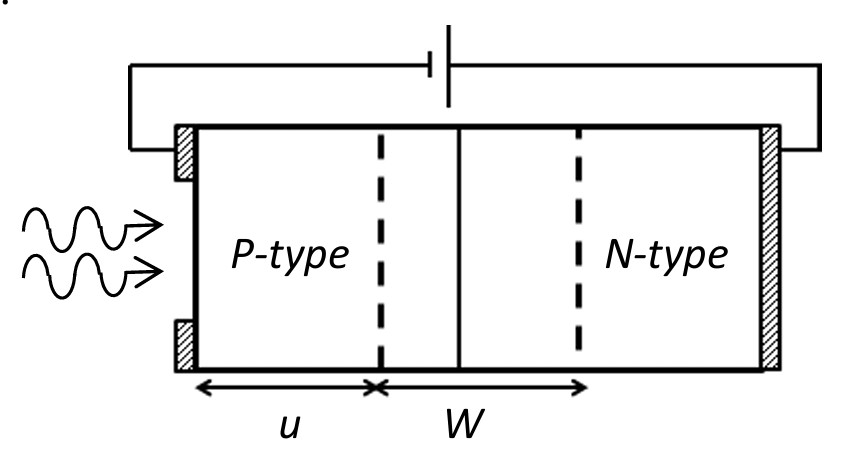
\includegraphics[width=0.52\linewidth]{../Figures/Sheet 8/q6.jpg}
\end{center}
(a) Sketch the distribution of the light power along the depth of penetration inside the photodetector starting from air.\\
(b) Calculate the following (1) The quantum efficiency, (2) The maximum detectable wavelength if the energy gap of silicon is 1.11 eV. (3) The responsivity. (4) The photocurrent.
\end{question}

\textbf{\large Solution --- Question 6}

\textbf{Physical Insight: Plotting the Power Decay}
This question forces us to visualize the "Photon Journey" mathematically. The light power doesn't decay smoothly from the very outside; it undergoes a discontinuous drop at the surface due to reflection, and then decays exponentially ($e^{-\alpha x}$) through both the dead zone and the active zone.

The given parameters are $n_1 = 1$ (air), $n_2 = 3.5$ (silicon), $W = 10\,\mu\text{m}$, $x_0 = 5\,\mu\text{m}$, $\lambda = 0.8\,\mu\text{m}$, $P_{\text{inc}} = 1.5\,\mu\text{W}$, and $\alpha = 800\,\text{cm}^{-1} = 8\times10^4\,\text{m}^{-1}$.

\textbf{(a) Power distribution sketch.}

First we establish the key power levels. At the air-silicon interface, the reflected fraction is:

\begin{equation*}
  R = \left(\frac{3.5 - 1}{3.5 + 1}\right)^2 = \left(\frac{2.5}{4.5}\right)^2 = 0.3086
\end{equation*}

so the power entering the silicon is $(1-R)P_{\text{inc}} = 0.6914\times1.5\,\mu\text{W} = 1.037\,\mu\text{W}$. This transmitted power decays exponentially through the p-type contact layer ($x_0 = 5\,\mu\text{m}$) and into the depletion region ($W = 10\,\mu\text{m}$). The power at the start of the depletion region ($x = x_0$) is:

\begin{equation*}
  P_1 = (1-R)P_{\text{inc}}\,e^{-\alpha x_0} = 1.037 \times e^{-(8\times10^4)(5\times10^{-6})} = 1.037\times e^{-0.4} = 1.037\times0.670 = 0.695\,\mu\text{W}
\end{equation*}

The power at the far edge of the depletion region ($x = x_0 + W$) is:

\begin{equation*}
  P_2 = (1-R)P_{\text{inc}}\,e^{-\alpha(x_0+W)} = 1.037\times e^{-(8\times10^4)(15\times10^{-6})} = 1.037\times e^{-1.2} = 1.037\times0.301 = 0.312\,\mu\text{W}
\end{equation*}

The distribution of power $P(x)$ inside the silicon starts at $(1-R)P_{\text{inc}}$ at $x=0^+$, drops with the exponential decay constant $1/\alpha = 12.5\,\mu\text{m}$ throughout both the contact layer and the depletion region, as illustrated in the figure below. Note that there is a discontinuous step at $x=0$ from $P_{\text{inc}}$ down to $(1-R)P_{\text{inc}}$ due to surface reflection.

\begin{figure}[H]
  \centering
  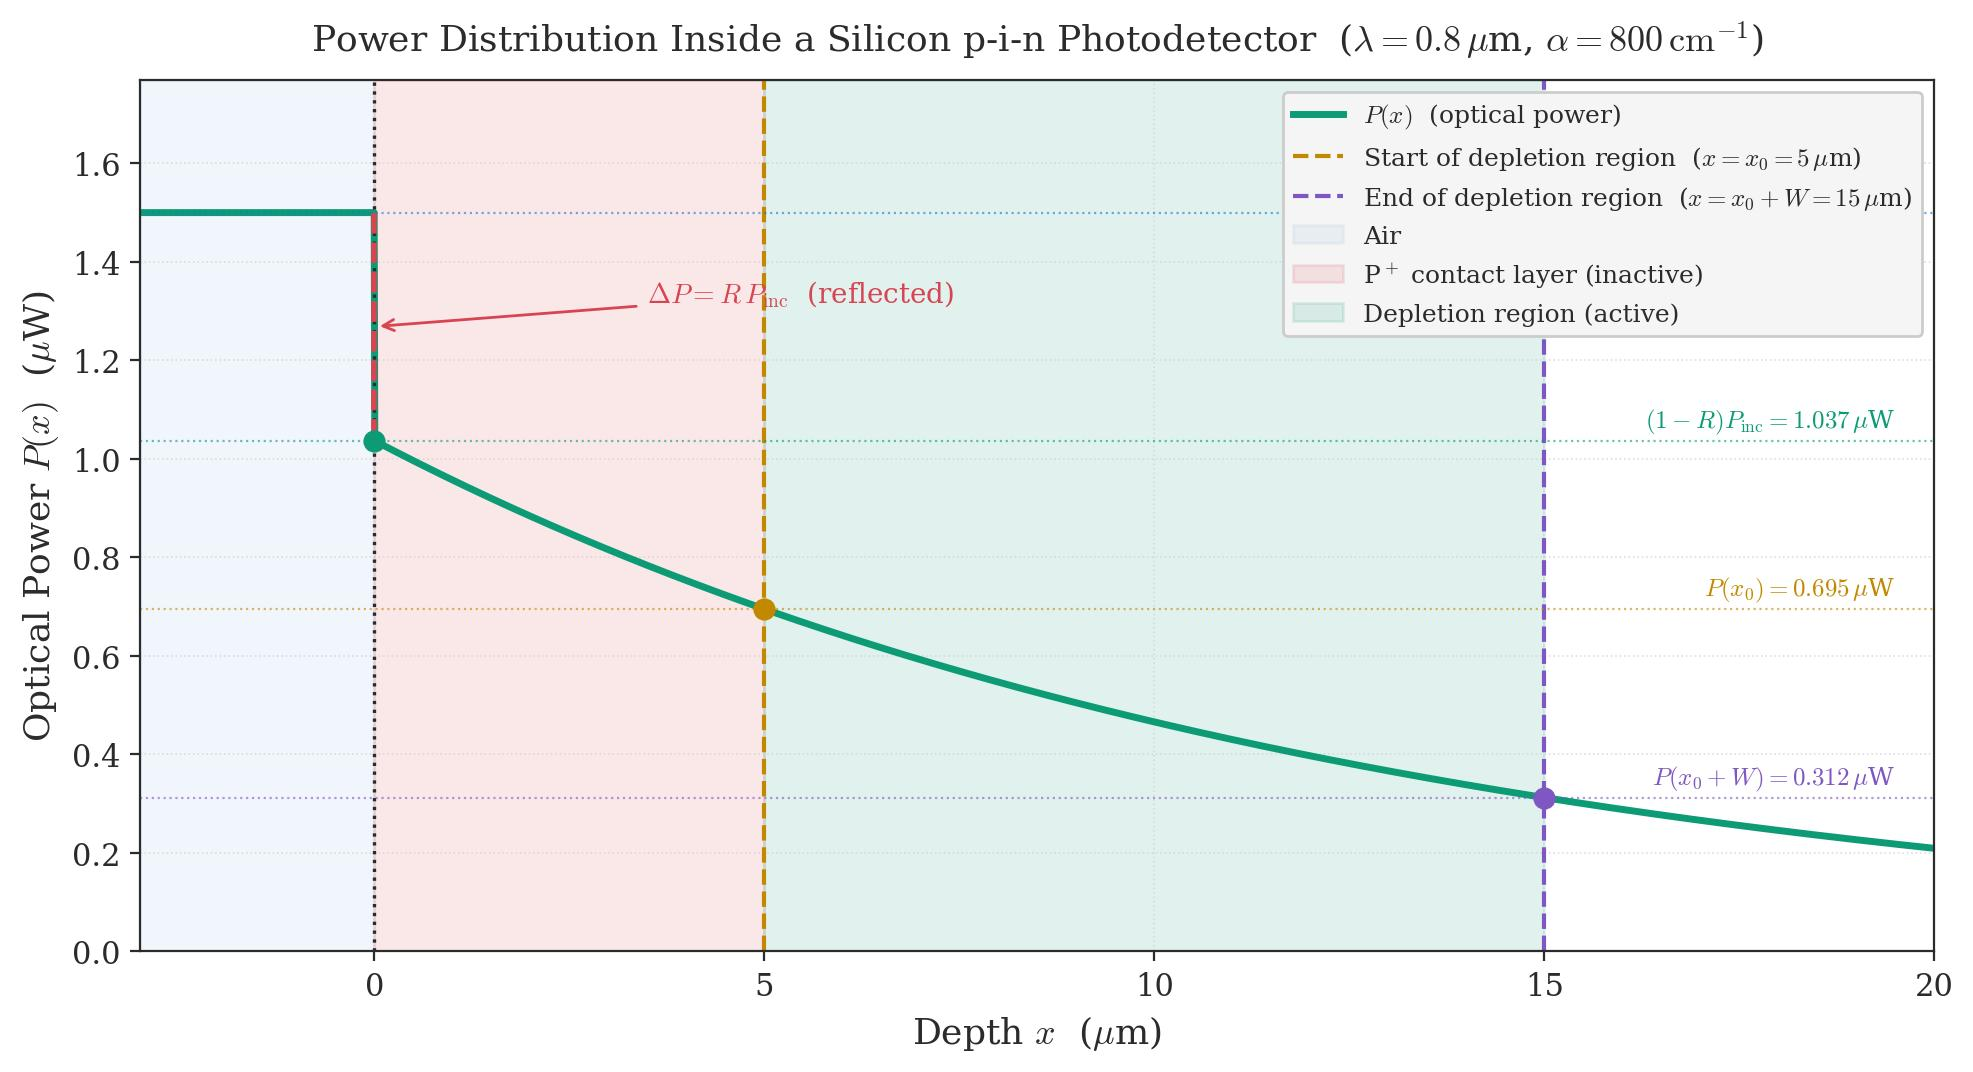
\includegraphics[width=0.72\textwidth]{../Figures/Sheet 8/q6_power_distribution.jpg}
\end{figure}

\textbf{(b)(1) Quantum efficiency.}

We will use the standard efficiency formula:
\begin{equation*}
  \eta = (1-R)(1 - e^{-\alpha L})\eta_{int}
\end{equation*}

We map the physical parameters directly:
\begin{itemize}
  \item \textbf{Reflection ($1-R$):} $0.6914$ (calculated in part a)
  \item \textbf{Active Layer Absorption $(1 - e^{-\alpha L})$:} Here $L = W = 10\,\mu\text{m}$, giving $1 - e^{-0.8} = 0.5507$
  \item \textbf{Internal Efficiency ($\eta_{int}$):} The survival fraction through the dead zone ($x_0 = 5\,\mu\text{m}$), which is $e^{-\alpha x_0} = e^{-0.4} = 0.6703$
\end{itemize}
Multiplying them together gives the total efficiency:
\begin{equation*}
  \eta = (0.6914) \times (0.5507) \times (0.6703) \approx 0.2552
\end{equation*}
\begin{equation*}
  \boxed{\eta = 25.5\%}
\end{equation*}

\textbf{(b)(2) Maximum detectable wavelength.}

Using the shortcut relating bandgap to wavelength:
\begin{equation*}
  \lambda_{\max} = \frac{1.24}{E_g[\text{eV}]} = \frac{1.24}{1.11}
\end{equation*}
\begin{equation*}
  \boxed{\lambda_{\max} = 1.117\,\mu\text{m}}
\end{equation*}

\textbf{(b)(3) Responsivity.}

Using the shortcut we rigorously derived in Question 4:
\begin{equation*}
  \mathcal{R} = \frac{\eta\lambda[\mu\text{m}]}{1.24} = \frac{0.2552 \times 0.8}{1.24}
\end{equation*}
\begin{equation*}
  \boxed{\mathcal{R} = 0.1646\,\text{A/W}}
\end{equation*}

\textbf{(b)(4) Photocurrent.}

\begin{equation*}
  I = \mathcal{R}\,P_{\text{inc}} = 0.1646 \times 1.5\,\mu\text{W}
\end{equation*}
\begin{equation*}
  \boxed{I = 0.2469\,\mu\text{A}}
\end{equation*}

\begin{question}[Question 7]
The P$^+$ contact layer of a Si p-i-n photodiode is 1 \si{\micro\meter} thick. Knowing that $\alpha = 5\times 10^4$ m$^{-1}$. Assume side illumination (a) Estimate the maximum quantum efficiency that can be expected at $\lambda=0.9$ \si{\micro\meter}.(b) Estimate the minimum thickness of the $\nu$-layer needed to ensure a quantum efficiency of 0.8 at this wavelength.
\end{question}

\textbf{\large Solution --- Question 7}

\textbf{Physical Insight: Side Illumination}
In a "side illumination" geometry, the light enters parallel to the junction rather than through the top surface. Here, the problem specifies that the light must travel transversely through $1\,\mu\text{m}$ of the $\text{P}^+$ contact layer before reaching the $\nu$-layer (the depletion region). We are told to ignore reflection ($R=0$). 
To maximize quantum efficiency, we want the active zone ($\nu$-layer) to be infinitely thick ($W \to \infty$) so that it catches every single photon that manages to survive the $\text{P}^+$ dead zone.

The given parameters are $x_0 = 1\,\mu\text{m}$ (P$^+$ contact layer thickness), $\alpha = 5\times10^4\,\text{m}^{-1}$, and $\lambda = 0.9\,\mu\text{m}$.

\textbf{(a) Maximum quantum efficiency.}

``Side illumination'' means the light enters from the side of the P$^+$ contact layer, traversing $x_0 = 1\,\mu\text{m}$ before hitting the active $\nu$-layer. We want the maximum efficiency, which occurs if the active zone is infinitely thick ($W \to \infty$) so no photons escape.

We will use the standard efficiency formula:
\begin{equation*}
  \eta = (1-R)(1 - e^{-\alpha L})\eta_{int}
\end{equation*}

We map the physical parameters directly:
\begin{itemize}
  \item \textbf{Reflection ($1-R$):} The problem tells us to ignore reflection, so $(1 - R) = 1$.
  \item \textbf{Active Layer Absorption $(1 - e^{-\alpha L})$:} Here the active layer $L$ is infinitely thick, so $(1 - e^{-\alpha \cdot \infty}) = 1 - 0 = 1$
  \item \textbf{Internal Efficiency ($\eta_{int}$):} The survival fraction through the dead zone ($x_0 = 1\,\mu\text{m}$), which is $e^{-\alpha x_0} = e^{-(5\times10^4)(1\times10^{-6})} = e^{-0.05} \approx 0.9512$
\end{itemize}
Multiplying them together gives the absolute maximum efficiency:
\begin{equation*}
  \eta_{\max} = 1 \times 1 \times 0.9512 = 0.9512
\end{equation*}
\begin{equation*}
  \boxed{\eta_{\max} = 95.12\%}
\end{equation*}

\textbf{(b) Minimum $\nu$-layer thickness for $\eta = 0.8$.}

We now want the total efficiency to be exactly $0.8$. The Reflection and Internal Efficiency fractions remain exactly the same as in part (a), so we just set up the full efficiency equation and isolate the Active Layer Absorption term:
\begin{equation*}
  \eta = (1-R)(1 - e^{-\alpha L})\eta_{int} = \eta_{\max} \bigl(1 - e^{-\alpha W}\bigr)
\end{equation*}
\begin{equation*}
  0.8 = 0.9512 \bigl(1 - e^{-\alpha W}\bigr) \quad\Longrightarrow\quad 1 - e^{-\alpha W} = \frac{0.8}{0.9512} = 0.8410
\end{equation*}
\begin{equation*}
  e^{-\alpha W} = 1 - 0.8410 = 0.1590
\end{equation*}
Taking the natural logarithm of both sides:
\begin{equation*}
  -\alpha W = \ln(0.1590) \approx -1.8388 \quad\Longrightarrow\quad W = \frac{1.8388}{5\times10^4\,\text{m}^{-1}}
\end{equation*}
\begin{equation*}
  \boxed{W = 36.78\,\mu\text{m}}
\end{equation*}



\begin{question}[Question 8]
A Si p$^+$-i-n$^+$ photodiode is 0.1 mm square. Its i-layer is 30 \si{\micro\meter} thick.\\
(a) Neglecting surface reflection and absorption in the contact layer, and taking $\alpha = 7\times 10^4$ m$^{-1}$ at $\lambda=0.82$\si{\micro\meter}, calculate the maximum quantum efficiency and responsivity at this wavelength.\\
(b) Calculate the transit times for electrons and holes across the i-region assuming that their average drift velocities are $7\times 10^4$ and $4\times 10^4$ m/s respectively.
\end{question}

\textbf{\large Solution --- Question 8}

\textbf{Physical Insight: Transit Time vs. Absorption}
This question explores the fundamental trade-off in photodiode design. 
\begin{itemize}
\item To absorb more light and increase efficiency, you want a very \textbf{wide} active zone ($W$).
\item But, to make the photodiode fast (high bandwidth), you want a very \textbf{narrow} active zone, so that the electrons and holes have less distance to travel (shorter transit time $t = W/v$).
\end{itemize}

The given parameters are $\text{Area} = 0.1\,\text{mm}^2$, $W = 30\,\mu\text{m} = 30\times10^{-6}\,\text{m}$, $R = 0$ (surface reflection neglected), $x_0 = 0$ (no contact-layer absorption), $\alpha = 7\times10^4\,\text{m}^{-1}$, $\lambda = 0.82\,\mu\text{m}$, $v_e = 7\times10^4\,\text{m/s}$, and $v_h = 4\times10^4\,\text{m/s}$.

\textbf{(a) Maximum quantum efficiency and responsivity.}

We will use the standard efficiency formula:
\begin{equation*}
  \eta = (1-R)(1 - e^{-\alpha L})\eta_{int}
\end{equation*}

We map the physical parameters directly:
\begin{itemize}
  \item \textbf{Reflection ($1-R$):} The problem says neglect surface reflection, so $(1 - R) = 1$.
  \item \textbf{Active Layer Absorption $(1 - e^{-\alpha L})$:} Here $L = W = 30\,\mu\text{m}$, giving $1 - e^{-(7\times10^4)(30\times10^{-6})} = 1 - e^{-2.1} = 1 - 0.1225 = 0.8775$
  \item \textbf{Internal Efficiency ($\eta_{int}$):} The problem says neglect contact layer absorption (no dead zone, $x_0 = 0$), so $\eta_{int} = e^0 = 1$.
\end{itemize}
Multiplying them together gives the overall efficiency:
\begin{equation*}
  \eta_{\max} = 1 \times 0.8775 \times 1 = 0.8775
\end{equation*}
\begin{equation*}
  \boxed{\eta_{\max} = 87.75\%}
\end{equation*}

For the responsivity, we use the shortcut formula from Question 4:
\begin{equation*}
  \mathcal{R} = \frac{\eta\lambda[\mu\text{m}]}{1.24} = \frac{0.8775 \times 0.82}{1.24} = \frac{0.71955}{1.24}
\end{equation*}
\begin{equation*}
  \boxed{\mathcal{R} = 0.5803\,\text{A/W}}
\end{equation*}

\textbf{(b) Transit times across the i-region.}

We will use the standard drift time formula:
\begin{equation*}
  \tau_{drift} = \frac{W}{v_d}
\end{equation*}

For the electrons:
\begin{equation*}
  \tau_{drift,e} = \frac{W}{v_e} = \frac{30\times10^{-6}\,\text{m}}{7\times10^4\,\text{m/s}} \approx 0.4286\times10^{-9}\,\text{s}
\end{equation*}
\begin{equation*}
  \boxed{\tau_{drift,e} = 0.4286\,\text{ns}}
\end{equation*}

For the holes:
\begin{equation*}
  \tau_{drift,h} = \frac{W}{v_h} = \frac{30\times10^{-6}\,\text{m}}{4\times10^4\,\text{m/s}} = 0.75\times10^{-9}\,\text{s}
\end{equation*}
\begin{equation*}
  \boxed{\tau_{drift,h} = 0.75\,\text{ns}}
\end{equation*}

\textbf{Conclusion:} The overall bandwidth of this photodiode is heavily limited by the slower carriers (the holes), which take $0.75\,\text{ns}$ to cross the active zone.

\begin{question}[Question 9]
Calculate the maximum values of load resistance that may be used when a photodiode having 1 pF self-capacitance is required to have an upper cutoff frequency of (a) 1 MHz (b) 1 GHz.
\end{question}

\textbf{\large Solution --- Question 9}

\textbf{Physical Insight: The RC Bandwidth Limit}
Even if the transit time of the carriers is extremely fast, the photodiode is still part of an electrical circuit. The internal capacitance of the diode junction ($C_D$) and the external load resistance ($R_B$) form a standard RC low-pass filter. If you want high-speed operation (GHz), you are forced to use a very tiny load resistor, which unfortunately produces a much weaker output voltage signal.

The given parameter is $C_D = 1\,\text{pF} = 10^{-12}\,\text{F}$.

\textbf{Step 1: The RC Bandwidth Formula}
The RC time constant ($\tau_{RC}$) of the photodiode circuit sets its bandwidth. The junction capacitance $C_D$ (where theoretically $C_D = \epsilon_s A / W$) and the load resistance $R_B$ form a simple first-order RC low-pass filter with time constant $\tau_{RC} = R_B C_D$. Its 3-dB cutoff frequency is:
\begin{equation*}
  f_{3\text{dB}} = \frac{1}{2\pi \tau_{RC}} = \frac{1}{2\pi R_B C_D} \quad\Longrightarrow\quad R_B = \frac{1}{2\pi f_{3\text{dB}} C_D}
\end{equation*}

\textbf{Step 2: Calculate for 1 MHz}
\begin{equation*}
  R_B = \frac{1}{2\pi (10^6) (10^{-12})} = \frac{1}{2\pi \times 10^{-6}} \approx 159.15\,\text{k}\Omega
\end{equation*}
\begin{equation*}
  \boxed{R_B = 159.2\,\text{k}\Omega}
\end{equation*}

\textbf{Step 3: Calculate for 1 GHz}
\begin{equation*}
  R_B = \frac{1}{2\pi (10^9) (10^{-12})} = \frac{1}{2\pi \times 10^{-3}} \approx 159.15\,\Omega
\end{equation*}
\begin{equation*}
  \boxed{R_B = 159.2\,\Omega}
\end{equation*}

The factor-of-1000 reduction in load resistance when going from MHz to GHz operation illustrates the fundamental bandwidth-efficiency trade-off in photodiode receivers: high bandwidth demands very low load resistance, which in turn reduces the voltage signal developed across the load and increases thermal noise.

\begin{question}[Question 10]
A conventional APD with gain G = 20 operates at a wavelength $\lambda = 1.55$ \si{\micro\meter}. If its responsivity at this wavelength is R = 12 A/W, calculate its quantum efficiency $\eta$. What is the photocurrent at the output of the device if a photon flux $\Phi = 10^{10}$ photons/s, at this same wavelength is incident on it?
\end{question}

\textbf{\large Solution --- Question 10}

\textbf{Physical Insight: Avalanche Multiplication}
An Avalanche Photodiode (APD) is operated under an extreme reverse bias. When a photon generates a primary electron, that electron is accelerated so violently by the electric field that it smashes into the crystal lattice, knocking loose more electrons (impact ionization). This creates an avalanche effect, multiplying the primary photocurrent by a gain factor $G$.

The given parameters are $G = 20$, $\lambda = 1.55\,\mu\text{m}$, $\mathcal{R}_{\text{APD}} = 12\,\text{A/W}$, and $\Phi_{\text{in}} = 10^{10}\,\text{photons/s}$.

\textbf{Step 1: Calculate Quantum Efficiency ($\eta$)}
An avalanche photodiode (APD) simply multiplies the raw responsivity of a normal PIN diode by the avalanche gain $G$.
\begin{equation*}
  \mathcal{R}_{\text{APD}} = G \cdot \mathcal{R}_{\text{PIN}} = G \left( \frac{\eta \lambda[\mu\text{m}]}{1.24} \right)
\end{equation*}
Rearranging to solve for the quantum efficiency:
\begin{equation*}
  \eta = \frac{1.24 \cdot \mathcal{R}_{\text{APD}}}{G \cdot \lambda[\mu\text{m}]} = \frac{1.24 \times 12}{20 \times 1.55} = \frac{14.88}{31} = 0.48
\end{equation*}
\begin{equation*}
  \boxed{\eta = 48\%}
\end{equation*}

\textbf{Step 2: Calculate Photocurrent ($I$)}
We are given the incoming photon flux ($\Phi_{\text{in}} = 10^{10}\,\text{photons/s}$), not the optical power. We must first find the energy of a single photon to find the total power. Using the energy shortcut:
\begin{equation*}
  E_{\text{photon}} = \frac{1.24}{\lambda[\mu\text{m}]}\,\text{eV} = \frac{1.24}{1.55}\,\text{eV} = 0.8\,\text{eV}
\end{equation*}
Convert this to Joules ($1\,\text{eV} = 1.6\times10^{-19}\,\text{J}$):
\begin{equation*}
  E_{\text{photon}} = 0.8 \times 1.6\times10^{-19} = 1.28\times10^{-19}\,\text{J}
\end{equation*}
The total optical power is the energy per photon times the number of photons per second:
\begin{equation*}
  P = \Phi_{\text{in}} \times E_{\text{photon}} = (10^{10}) \times (1.28\times10^{-19}) = 1.28\times10^{-9}\,\text{W} = 1.28\,\text{nW}
\end{equation*}
Now use the responsivity to find the final photocurrent:
\begin{equation*}
  I = \mathcal{R}_{\text{APD}} \times P = 12\,\text{A/W} \times 1.28\,\text{nW}
\end{equation*}
\begin{equation*}
  \boxed{I = 15.36\,\text{nA}}
\end{equation*}

\begin{question}[Formative Assignment Problem]
Show that a carrier of charge $Q$ moving with a velocity $v(t)$ in the $x$-direction inside a semiconductor material of width $W$ under the influence of an electric field $E$ creates a current in the external circuit given by $i(t) = -\frac{Q}{W} v(t)$. This formula is known as Ramo's theorem. (Hint: If the charge moves a distance $dx$ in the time $dt$, then the work done by the electric field on the charge $-QE dx$ must equal the energy $i(t) V dt$ provided by the external circuit). Use Ramo's theorem to show that an electron-hole pair generated at any point $x$ within the semiconductor material produces a total charge of $e$ (not $2e$) in the external circuit.
\end{question}

\textbf{\large Solution --- Formative Assignment: Ramo's Theorem}

\textbf{Physical Insight: The Illusion of Charge Collection}
It is incredibly tempting to think: "If a photon creates 1 electron and 1 hole, and they both travel to the opposite terminals, didn't I just collect $2e$ of charge?"
\textbf{No!} Ramo's Theorem proves that this is an illusion. The current in the wires isn't waiting for the electron to arrive. The moment the electron starts moving, it pushes charge through the external wires via the electric field. By using the universal law of \textbf{Energy Conservation}, we can prove that the total work done by the battery moving the entire electron-hole pair sums perfectly to exactly $1e$ of charge, regardless of where in the device the photon was absorbed.

\textbf{Part 1 — Deriving Ramo's theorem.}

Consider a carrier of charge $Q$ moving with instantaneous velocity $v(t)$ in the $x$-direction inside the semiconductor slab of width $W$. A uniform electric field $E = V/W$ exists across the slab (where $V$ is the applied voltage). When the carrier moves a small distance $dx$ in time $dt$, the work done by the electric field on the charge is:

\begin{equation*}
  dW_{\text{field}} = (-QE)\,dx = -\frac{QV}{W}\,dx
\end{equation*}

The negative sign reflects the convention that the force on charge $Q$ in field $E$ is $F = QE$, and if $Q$ is an electron ($Q = -e$), the force is in the direction opposing positive field direction. The energy supplied by the external circuit to maintain the voltage $V$ across the terminals while current $i(t)$ flows is:

\begin{equation*}
  dW_{\text{ext}} = i(t)\,V\,dt
\end{equation*}

By energy conservation, the work done by the field on the carrier must be supplied by the external circuit:

\begin{equation*}
  dW_{\text{ext}} = -dW_{\text{field}} \quad\Longrightarrow\quad i(t)\,V\,dt = \frac{QV}{W}\,dx
\end{equation*}

Cancelling $V$ from both sides and dividing by $dt$:

\begin{equation*}
  i(t) = \frac{Q}{W}\cdot\frac{dx}{dt} = \frac{Q}{W}\,v(t)
\end{equation*}

For an electron ($Q = -e$, $e > 0$) drifting in the direction of the field:

\begin{equation*}
  \boxed{i(t) = -\frac{Q}{W}\,v(t)}
\end{equation*}

This is Ramo's theorem. The key insight is that the current in the external circuit depends only on the instantaneous carrier velocity and the device geometry — not on the position of the carrier. Even before the carrier reaches the contact, it induces current in the external circuit.

\textbf{Part 2 — Total charge for an electron-hole pair.}

Suppose an electron-hole pair is photogenerated at position $x$ inside the slab of width $W$ (where $0 \leq x \leq W$). Under the applied field, the electron drifts toward the positive terminal and the hole drifts toward the negative terminal.

The total charge collected from each carrier is found by integrating the induced current over the transit time. For the electron, which must travel a distance $(W - x)$ to reach the positive contact at drift velocity $v_e$:

\begin{equation*}
  Q_e = \int_0^{t_e} i_e(t)\,dt = \frac{e}{W}\cdot v_e \cdot t_e = \frac{e}{W}\cdot(W-x) = e\,\frac{W-x}{W}
\end{equation*}

For the hole, which must travel a distance $x$ to reach the negative contact at drift velocity $v_h$:

\begin{equation*}
  Q_h = \int_0^{t_h} i_h(t)\,dt = \frac{e}{W}\cdot v_h\cdot t_h = \frac{e}{W}\cdot x = e\,\frac{x}{W}
\end{equation*}

The total charge delivered to the external circuit by both carriers is:

\begin{equation*}
  Q_{\text{total}} = Q_e + Q_h = e\,\frac{W-x}{W} + e\,\frac{x}{W} = e\,\frac{(W-x)+x}{W} = e\cdot\frac{W}{W}
\end{equation*}

\begin{equation*}
  \boxed{Q_{\text{total}} = e}
\end{equation*}

The result is independent of the generation position $x$ — no matter where in the device the pair is created, the total charge induced in the external circuit is exactly $e$, not $2e$. The factor of 2 does not arise because the two carriers travel in opposite directions and their individual contributions always sum to give a total displacement current of exactly one electron charge. This is the profound elegance of Ramo's theorem applied to photodetectors.
